%!TEX root = ./../thesis.tex

\chapter{Experiments}
\label{c:experiments}
In order to evaluate the current performance of the framework, a series of experiments has been conducted.
The experiments are divided into two parts, where the first part focuses on the assessment of the overall algorithm performance when executing machine learning algorithms in a distributed fashion.
For comparison Apache Spark is used, as the system is currently the state-of-the-art in distributed machine learning as well as a non-parallel baseline implementation.
Besides the evaluation of the current status of the framework another motivation behind this set of experiments is to prove the usefulness of the programming model.
The second set of experiments tries to quantify how different facets of consistency management affect the algorithm performance.
Therefore the impact of communication frequency, synchronization strategy as well as various filter and merging strategies on the overall algorithm performance is evaluated.

\section{Experiment Setup}
As the algorithm for comparison, distributed lasso linear regression within the CoCoA framework is used as described in section \ref{ss:cocoa}.
Based on the generic form of convex optimization problems described in (\ref{eqn:lin_loss}), lasso linear regression is represented by
\begin{equation}
f_\alpha = \frac{1}{2} \parallel D\alpha - y \parallel^2_2
\label{eqn:lasso}
\end{equation}
and
\begin{equation}
r(\alpha) = \lambda \parallel \alpha \parallel_1
\label{eqn:lasso_reg}
\end{equation}
where $\alpha$ is the weight vector, $D$ resembles the input data together with the output $y$ and $\lambda$ is the regularization constant.
Simple randomized coordinate descent is used as the local solver within the CoCoA framework, as described in (\ref{alg:scd}).
As a measure for the overall algorithm performance the distance to the optimal primal solution is used. This optimal value is calculated by running all methods for a large number of iterations (until the algorithm is converged) and then selecting the smallest primal value amongst the results.

In order to show the algorithm performance from different perspectives, two datasets with different properties such as ratio between number of examples and feature size as well as sparsity are used, as can be seen in Table \ref{tab:datasets}.
In BSP the runtime is measured on a per iteration basis on the driver for Apache Spark as well as the framework.
This includes scheduling of computation and execution.
When running stale synchronous parallel (SSP) and total asynchronous parallel (TAP) the runtime is measured for each node and iteration independently and the overall runtime is set by the best performing node.
For a better comparison between systems the data loading and setup stage is not accounted to the overall runtime.
\begin{table}[h]
\begin{center}
\begin{tabular}{ | c | c | c | c |}
\hline
\textbf{Dataset} & \textbf{Training Size} & \textbf{Feature Size} & \textbf{Sparsity} \\ \hline
epsilon & 400 K & 2 K & 1.0 \\ \hline
URL & 2.4 M & 3.2 M & 3.5e-5 \\
\hline
\end{tabular}
\end{center}
\caption{Datasets for Empirical Evaluation}
\label{tab:datasets}
\end{table}

The cluster itself consists of 8 machines with each machine equipped with 16 GB of RAM and 8 Intel Xeon E3-1230 V2 CPUs running at 3.30 GHz.
All nodes are connected via 1 GBit Ethernet.
Distributed experiments running Apache Spark and the framework use 8 machines if not stated otherwise.
As a baseline, a single-core implementation of the algorithm is used.

\section{Algorithm Performance}
For assessment of the algorithm performance in comparison to Apache Spark and the baseline, lasso regression is run on the epsilon and URL dataset with bulk synchronous parallel synchronization (BSP) as discussed in Section \ref{ss:synchronization}.
The algorithm hyper-parameters $\gamma$ and $\lambda$ have been tuned for best performance and are set to 1.0 and 1e-5, respectively, on both datasets.
In order to provide a better comparability, the parameter $H$ indicating the fraction of the local features that are refined during an iteration is set to 1.0 for all systems.
Therefore at each iteration the whole feature set is refined before each unit communicates its shared parameter $v$ to its corresponding replicas. 
\begin{figure}[ht]
\centering
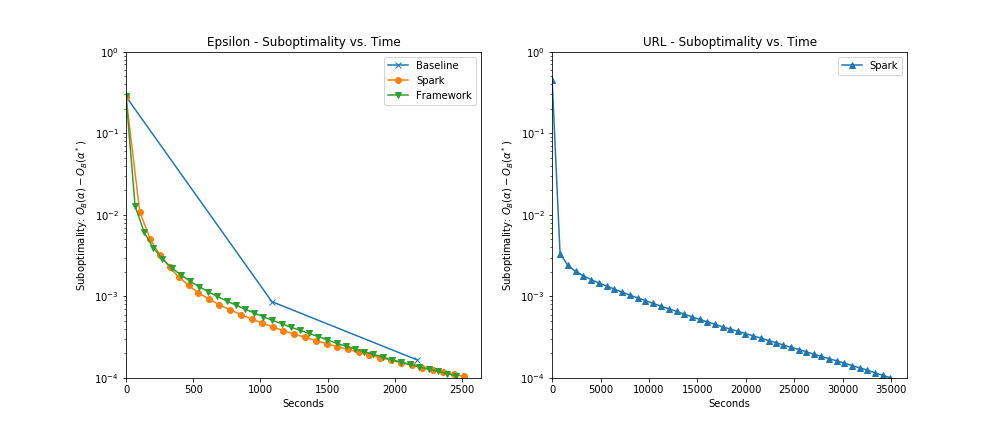
\includegraphics[width=1.0\textwidth]{img/overall_perf_cmp.png}
\caption{Overall Algorithm Performance Comparison}
\label{fig:algo_perf_cmp}
\end{figure}
From Figure \ref{fig:algo_perf_cmp} can be seen that both systems perform better than the baseline on the epsilon dataset.
It should be noted that in comparison to the distributed implementations the baseline still performs quite well due to the fact that the dataset is small enough to fit into a single machines memory.
But as soon as the data size grows grows beyond this size, only the distributed systems can scale with the data size.
Furthermore it can be seen from the comparison between the framework and Apache Spark that the algorithm distributed with the framework converges faster.
This behavior stems from the fact that the epsilon dataset has a small number of features, which are then distributed over multiple machines for parallel refinement, resulting in a small iteration runtime.
As already mentioned in Section \ref{s:distributed_ml}, this common distributed machine learning procedure of quick refinements followed by communicating the current progress among all participating workers is not a good fit for a data-flow system like Apache Spark.
In contrast to the epsilon dataset, the baseline implementation gives similar results to the distributed systems.
The reason is for this behavior is twofold.
First, due to the large number of samples in the dataset the resulting parameter vector $v$ that needs to be communicated over the network grows quite large.
This increases the time spent on communication and therefore decreases the available time for computation of parameter refinements.
Second, as the algorithm progresses the updates become smaller, which also lowers the benefit of sharing the local progress among the parallel workers.
In order to mitigate this behavior, multiple filtering strategies will be evaluated in Section \ref{ss:filtering_strategy}.

\section{Consistency Management}
As consistency management is the key part of an efficient distributed machine learning system, this section tries to quantify the impact of multiple consistency management related properties on the algorithm performance.
As discussed in Section \ref{s:state_centric_comp_centric}, state-level consistency can be maintained by altering the local update communication frequency between unit replicas, while control-flow consistency can be achieved by choosing the proper synchronization strategy.
Therefore these two properties are evaluated in different configurations, followed by an evaluation of different filtering strategies as discussed in Section \ref{s:strategies}.

\subsection{Communication Frequency}
Evaluating the correlation between algorithm performance and communication frequency is done using lasso regression on the epsilon and URL dataset with stale synchronous parallel synchronization (SSP) as previously discussed in Section \ref{ss:synchronization}.
As a baseline the algorithm performance is compared to Apache Spark.
The hyper-parameters $\gamma$ and $\lambda$ are again set to 1.0 and 1e-5 for both datasets and the staleness threshold $\tau$ is set to 3.
In this experiment the parameter $H$ refers to the fraction of the dataset that is processed for parameter refinement of $\alpha$ before the shared parameter vector $v$ is communicated to the participating workers.
\begin{figure}[ht]
\centering
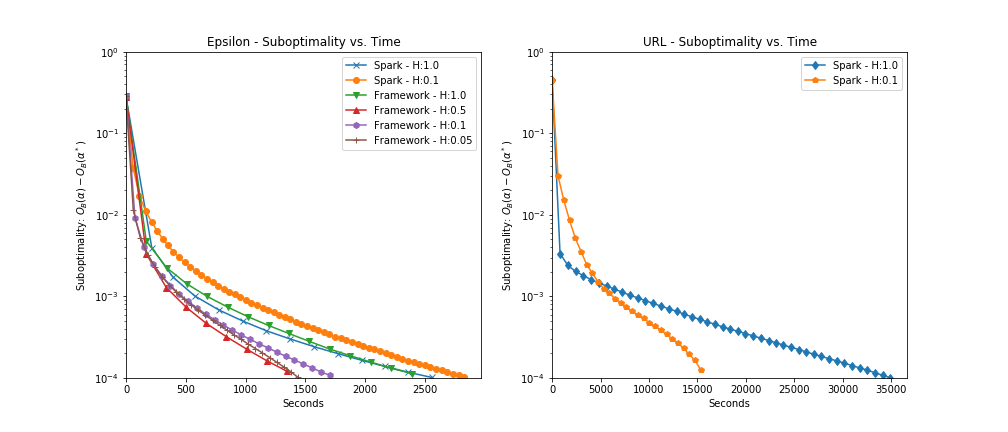
\includegraphics[width=1.0\textwidth]{img/comm_freq_cmp.png}
\caption{Communication Frequency Comparison}
\label{fig:comm_freq_cmp}
\end{figure}
As depicted in Figure \ref{fig:comm_freq_cmp}, increasing the communication frequency within the framework on the epsilon dataset increases the algorithm performance considerably, with the best results observed for $H$ set to 0.1.
The reason this works so well is again twofold.
First, though the amount of data to be communicated by each worker increases by a factor of 10, sharing progress as early as possible increases the algorithm performance as discussed in Section \ref{ss:consistency}.
Second, due to the small number of samples in the dataset the resulting amount of communication is still small enough not to interfere with the actual parameter refinement computation.
On the other hand, with the implementation on Apache Spark using $H=0.1$ the algorithm converges slowly.
The reason is that the increase in communication frequency also significantly increases the overhead required for aggregation and communication of the shared parameter vector as well as scheduling of the next iteration, even though the amount of data to be communicated is small.
Repeating the same experiments with the URL dataset shows that increasing the communication frequency degrades the algorithm performance on the framework as well.
Again the reason for this behavior stems from the fact that the increased dataset size drastically increases the amount of parameter updates to be communicated and therefore the best choice for $H$ is in this case 1.0.

\subsection{Synchronization Strategy}
In this experiment the influence of the synchronization strategies discussed in Section \ref{ss:synchronization} on the algorithm performance is investigated.
Similar to the previous experiments, the hyper-parameters $\gamma$ and $\lambda$ are set to 1.0 and 1e-5.
Furthermore the staleness threshold is set to 1, 3 and infinity for BSP, SSP and TAP, respectively.
\begin{figure}[ht]
\centering
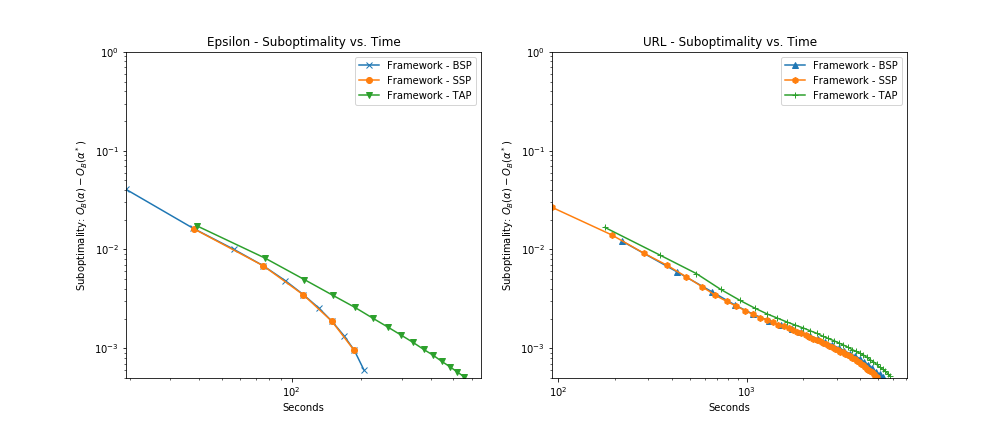
\includegraphics[width=1.0\textwidth]{img/sync_strat_cmp.png}
\caption{Synchronization Strategy Comparison}
\label{fig:sync_strat_cmp}
\end{figure}
From Figure \ref{fig:sync_strat_cmp} can be seen that BSP and SSP perform equally well on the epsilon dataset, whereas TAP converges significantly slower.
As already discussed in Section \ref{ss:synchronization}, the reason that TAP performs worse than BSP and SSP is due to fact that workers receive parameter updates from very different algorithm progress due to the asynchronicity in update computation.
These stale updates can spoil the solution and therefore decrease the overall algorithm performance.
This is even amplified by the small iteration runtime that increases the likelihood of the workers quickly diverging in their algorithm progress.
In contrast, the URL dataset has a long iteration runtime and it is therefore less likely to observe a severe divergence in iterations between parallel workers.
